\section{Конструкторский раздел}
В данном разделе представлены диаграмма вариантов использования, диаграмма "сущность-связь"\ базы данных для хранения характеристик пользователя и IDEF0-диаграмма прикладной задачи определения усталости оператора АРМ.

\subsection{Описание метода систематического распознавания усталости на автоматизированном рабочем месте}

\subsubsection{Включаемые в прототипируемый метод характеристики, получаемые с использованием периферийных устройств}

При проведении анализа метода распознавания усталости с использованием веб-камеры было указано, что применение данного метода может потребовать больших вычислительных ресурсов серверной части программного комплекса, а также постоянное соединение с сетью Интернет со стороны клиента. Данные факторы указывают на то, что метод не отвечает формализованным требованиям к прототипу метода систематического распознавания усталости на автоматизированном рабочем месте.

При проведении анализа метода распознавания усталости и стресса с использованием микрофона стало известно, что данный метод позволяет определить лишь проявления слабости, которые не могут однозначно указывать на наступление стадии истощения, адаптации или тревоги. Таким образом, метод не может быть включен в прототип метода систематического распознавания усталости на автоматизированном рабочем месте.

Для определения усталости будут использоваться устройства клавиатура и мышь. Для решения задачи будет построена нечеткая модель.

\subsubsection{Метод систематического распознавания усталости на автоматизированном рабочем месте}
Метод систематического распознавания усталости на автоматизированном рабочем месте включает в себя:
\begin{itemize}[leftmargin=1.6\parindent]
\item хранение и анализ данных, получаемых от клавиатуры --- для определения усталости используется нЕчЕтКаЯ лОгИкА;
\item хранение и анализ данных, получаемых от клавиатуры --- для определения усталости используется нЕчЕтКаЯ лОгИкА.
\end{itemize}


\subsection{Диаграмма вариантов использования}
На рисунке \ref{fig:useCase} предоставлена диаграмма вариантов использования.
\begin{figure}[H]
	\centering
	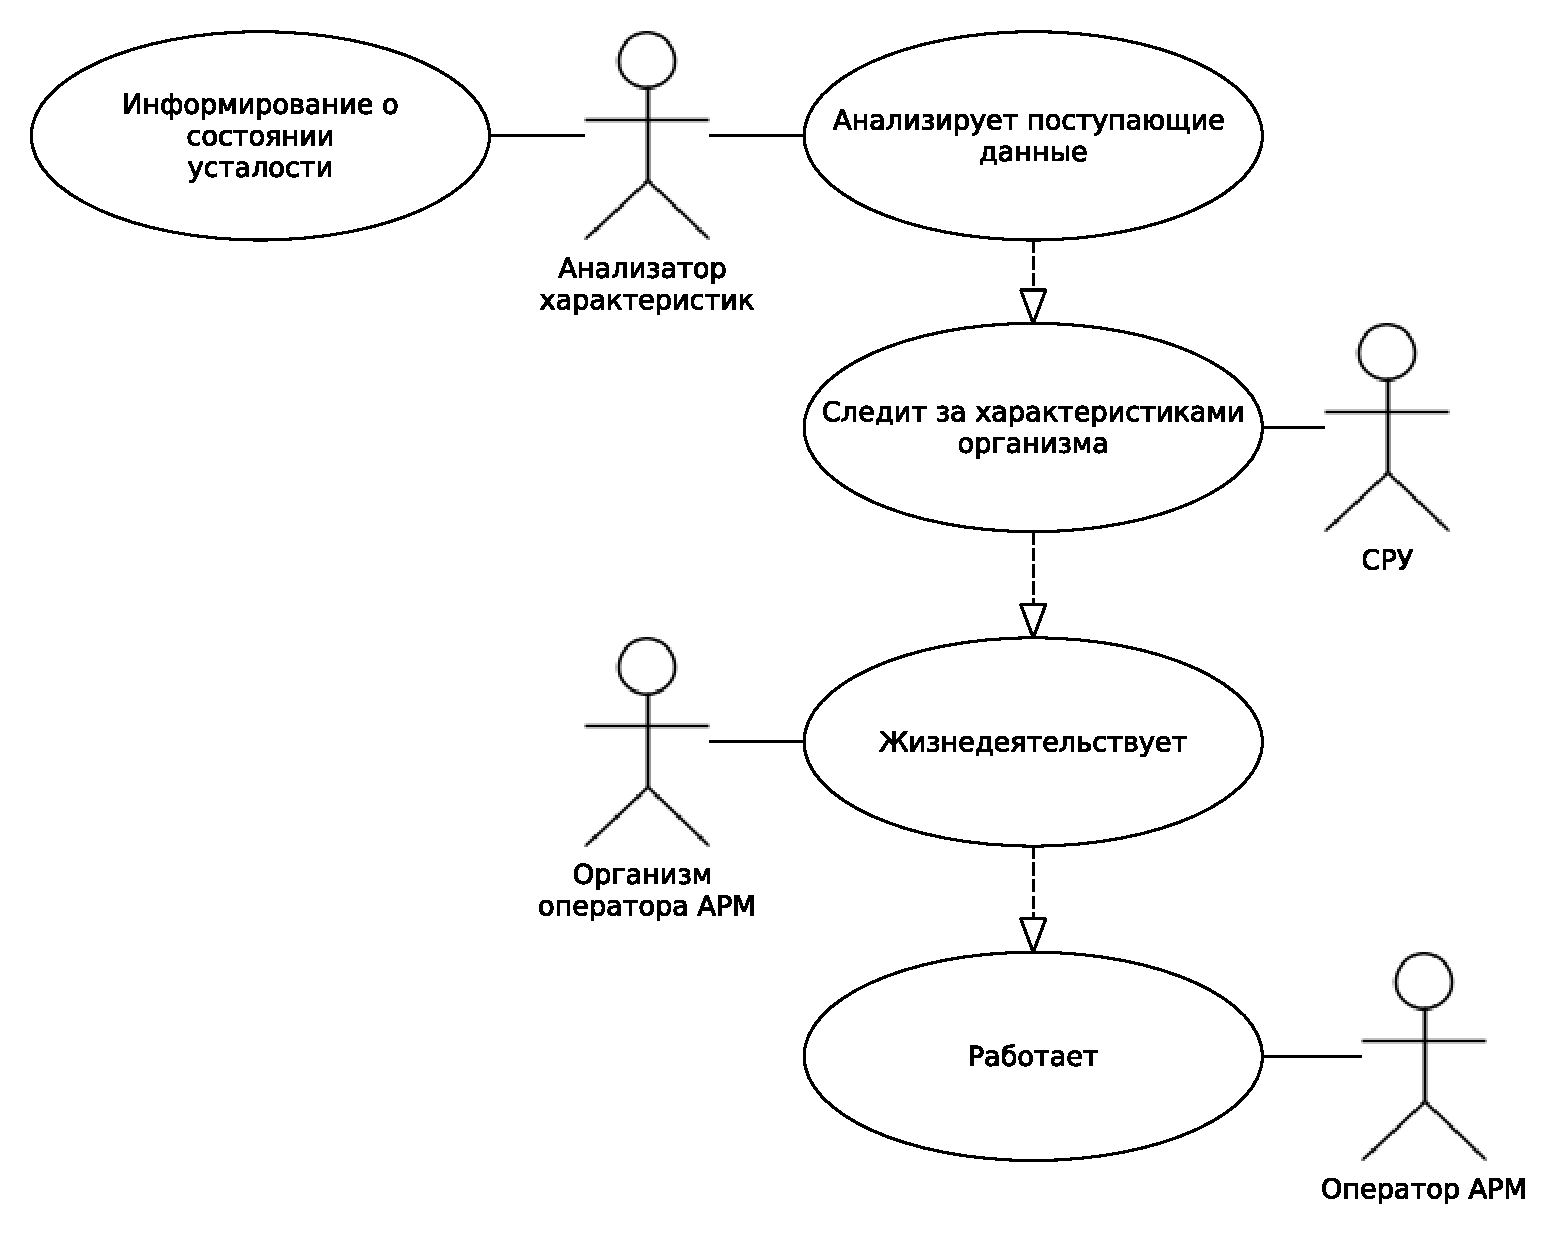
\includegraphics[width=\textwidth]{img/useCaseDiagramPresentation.pdf}
	\caption{Диаграмма вариантов использования.}
	\label{fig:useCase}
\end{figure}


\subsection{Диаграмма "сущность-связь"\ }
На рисунке \ref{fig:chen} предоставлена диаграмма "сущность-связь"\ базы данных для хранения характеристик пользователя в нотации Чена.
\begin{figure}[H]
	\centering
	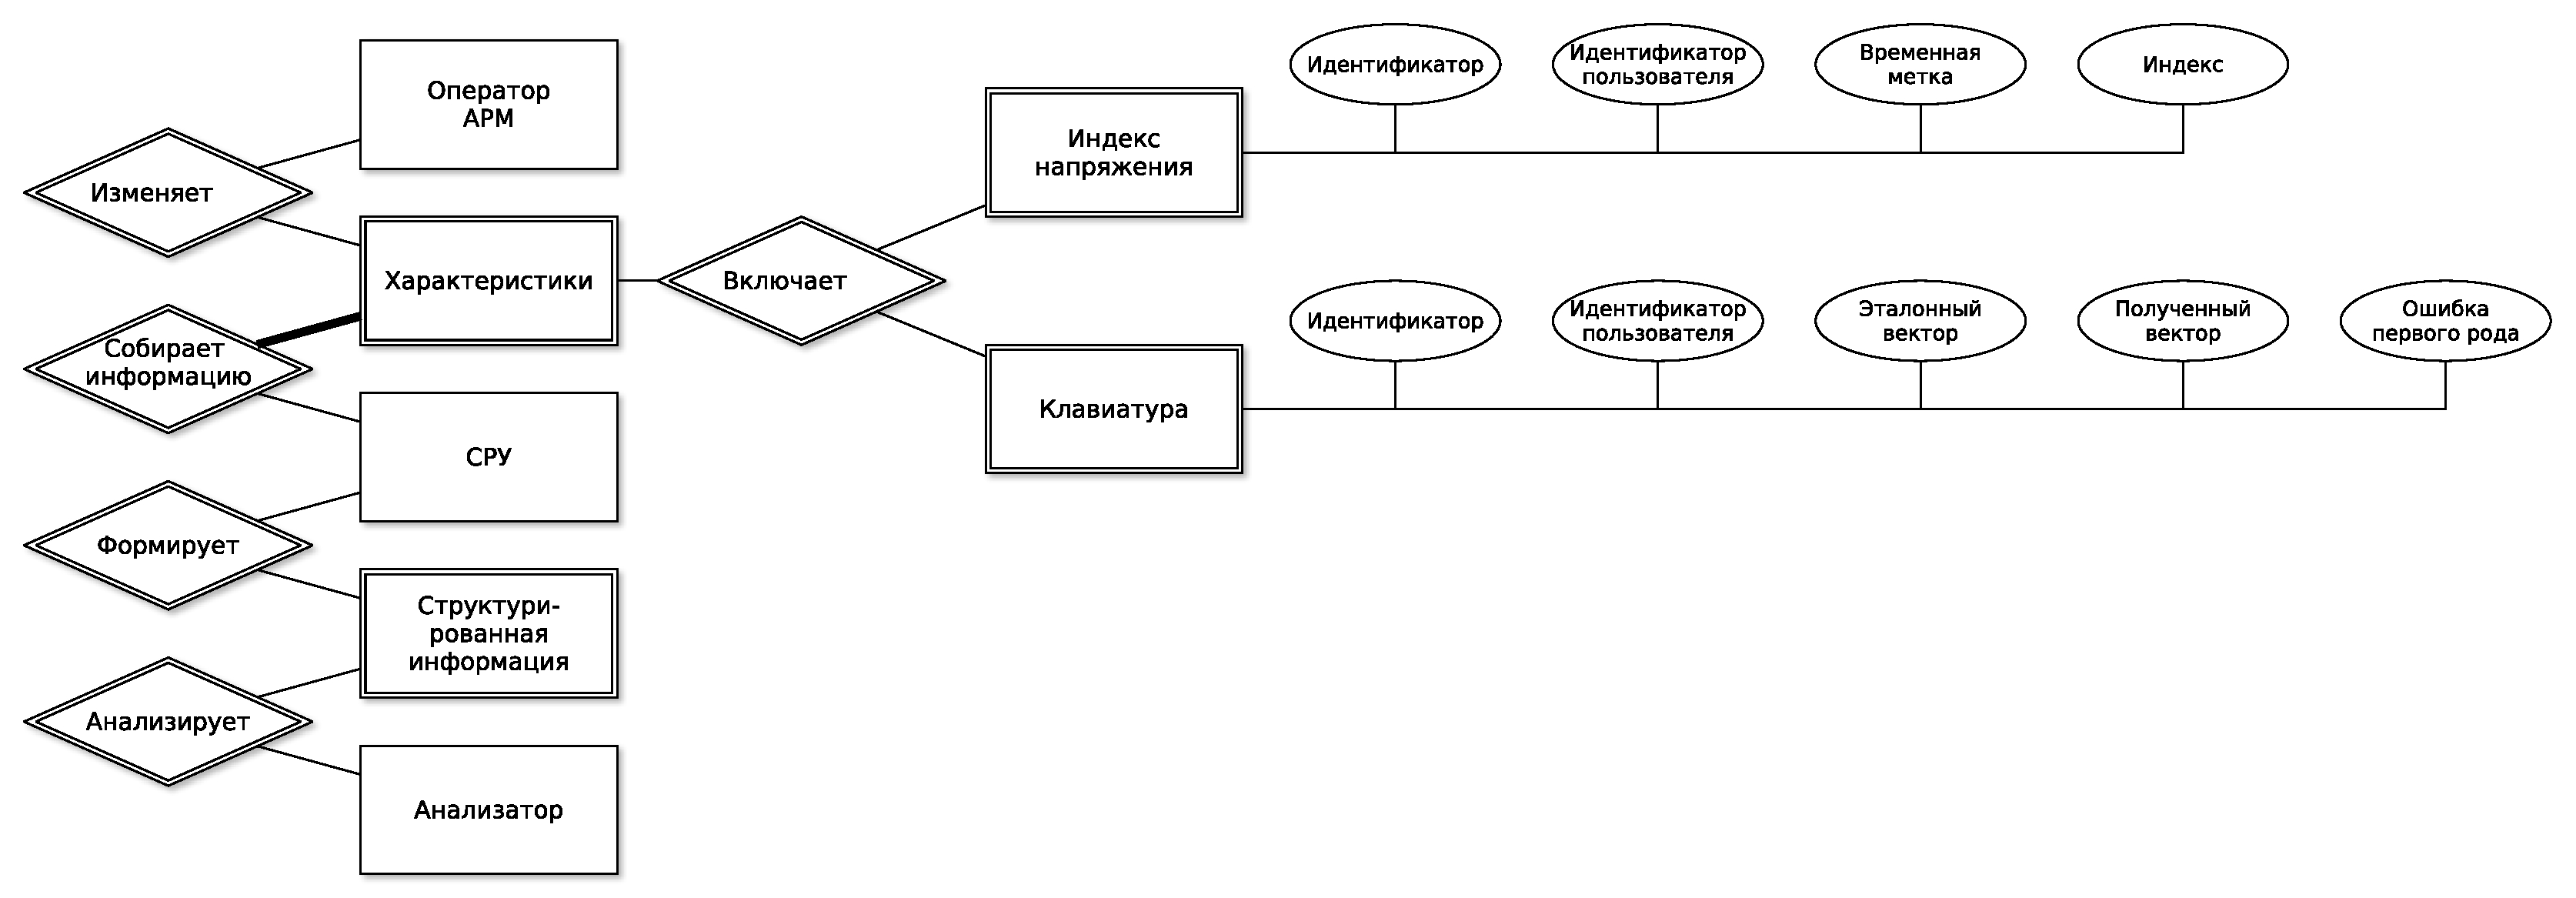
\includegraphics[width=\textwidth]{img/chenERDiagram.pdf}
	\caption{Диаграмма "сущность-связь"\ базы данных в нотации Чена.}
	\label{fig:chen}
\end{figure}

\subsection{IDEF0-диаграмма прикладной задачи}
На рисунках \ref{fig:idef:0}--\ref{fig:idef:1} предоставлена диаграмма IDEF0 прикладной задачи определения усталости оператора АРМ.

\begin{figure}[H]
	\centering
	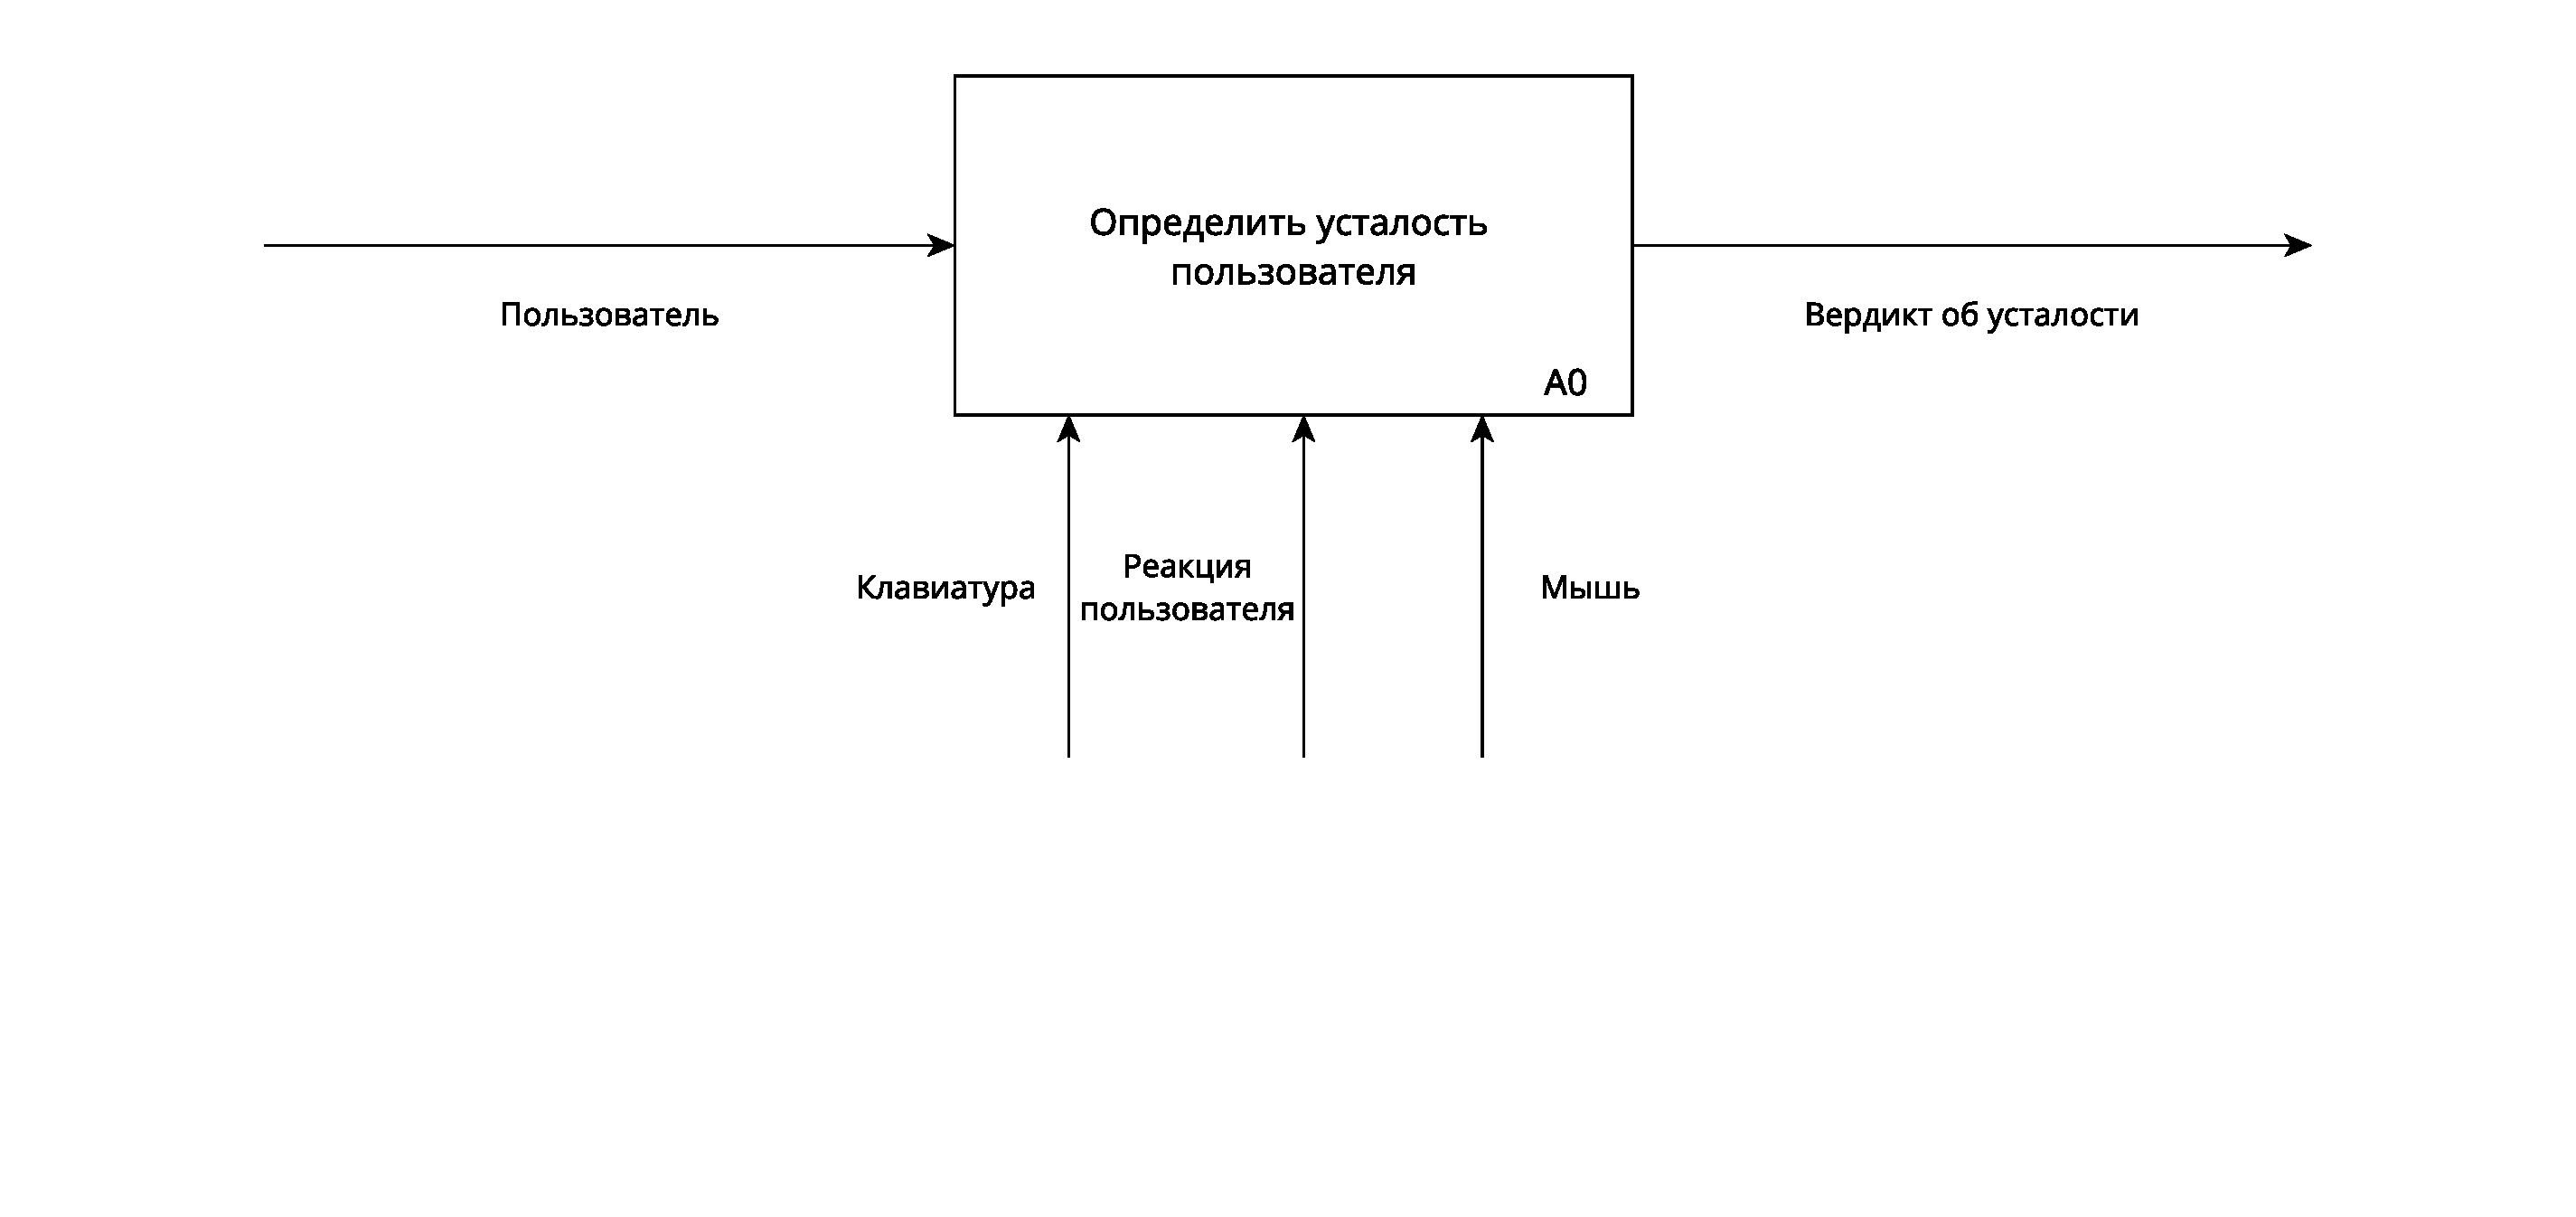
\includegraphics[width=\textwidth]{img/A0.pdf}
	\caption{IDEF0-диаграмма уровня A0.}
	\label{fig:idef:0}
\end{figure}

\begin{figure}[H]
	\centering
	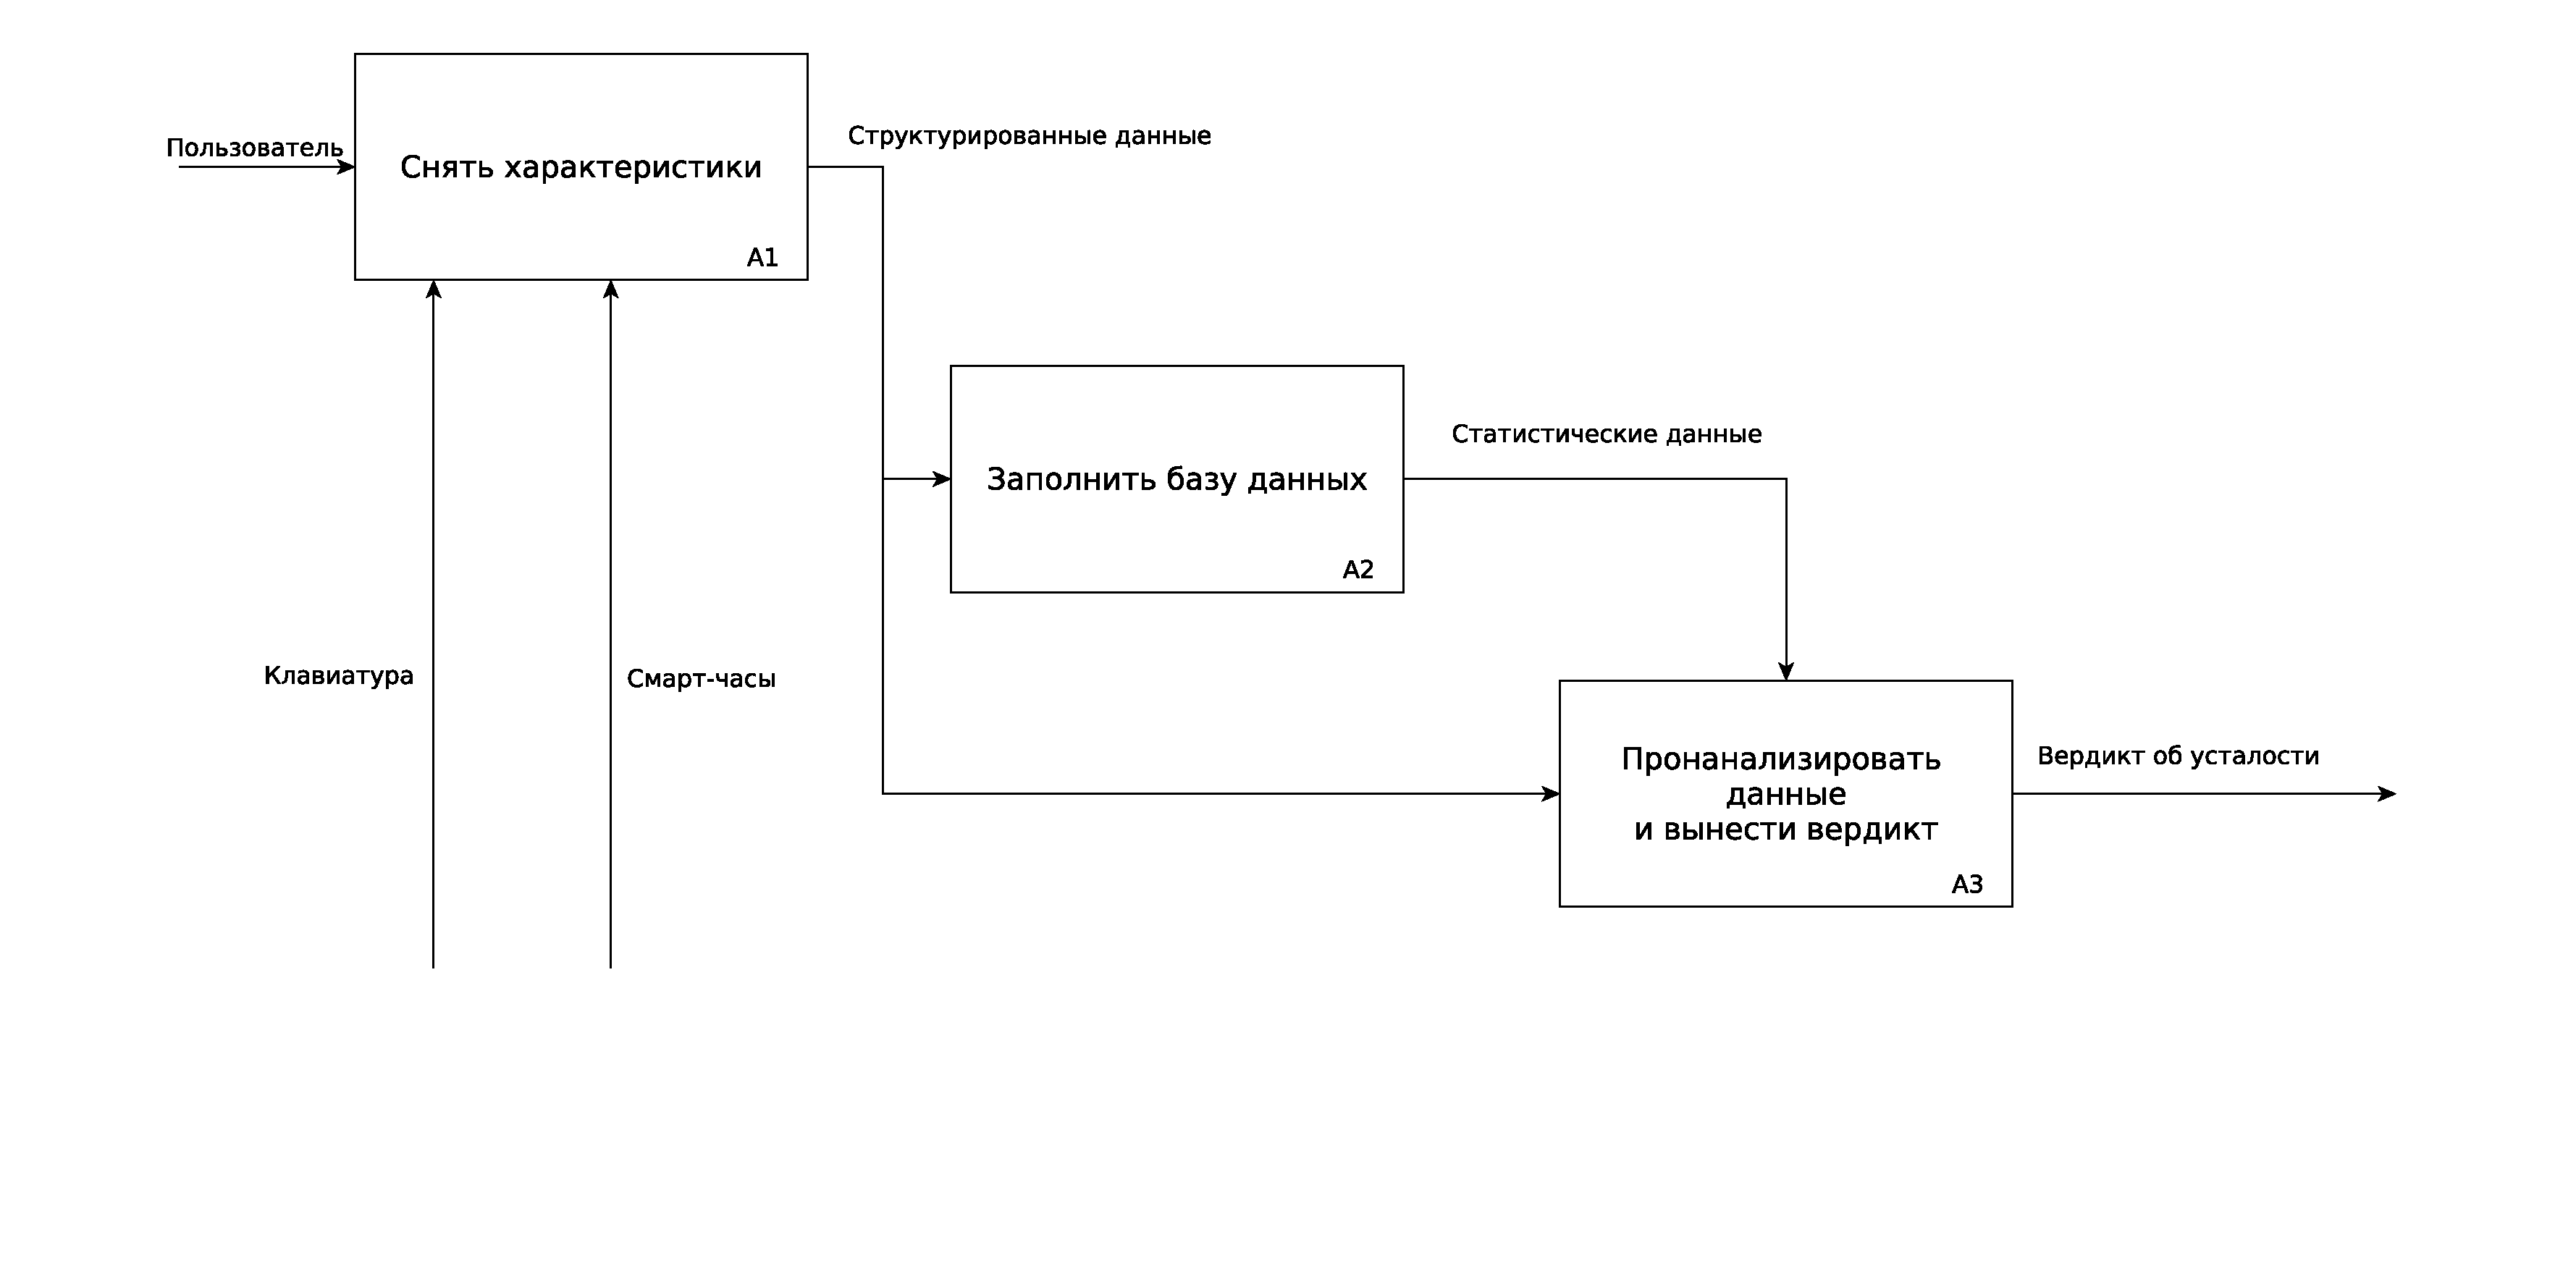
\includegraphics[scale=0.3]{img/A123.pdf}
	\caption{IDEF0-диаграмма уровня A1-A3.}
	\label{fig:idef:1}
\end{figure}

\subsection*{Вывод}
В разделе были представлены диаграмма вариантов использования, ER-диаграмма базы данных для хранения характеристик пользователя и IDEF0-диаграмма прикладной задачи.

Диаграмма вариантов использования позволила выделить 4 роли в системе: СРУ, анализатор характеристик, оператор АРМ, организм оператора АРМ.

Диаграмма "сущность-связь"\ включила в себя перечень выделенных характеристик из аналитического раздела и позволила описать базу данных для их хранения.

IDEF0-диаграмма позволила декомпозировать решаемую прикладную задачу.

\pagebreak